\documentclass[svgnames, table, 10pt, aspectratio=169]{beamer} % aspectratio=1610, 149, 54, 43 et 32.]{beamer}
\usepackage{ae,lmodern}
\usepackage[english]{babel}  % package pour langue française
\usepackage[utf8]{inputenc} % compilation des mots accentués
\usepackage[T1]{fontenc}      % césure correcte des mots accentués 
\usepackage{eso-pic,rotating,graphicx} % insertion d'images et manipulation de la position
\usepackage{xcolor}
\usepackage[font=scriptsize]{caption}
\usepackage{subcaption} % utilisation d'une légende intermédiaire dans le cas d'une image multiple
\usepackage{url} % utilisation des liens url (utilisation dans le cas de la bibliographie par exemple
\usepackage{tcolorbox,listings} % coloration du texte et possibilité d'inclure blocs de codes
\usepackage{geometry} % customisation des layouts de page (marges, bordures, espacements)
\usepackage{amssymb} % caractères mathématiques
\usepackage{multirow, makecell} % tableau sur plusieurs colonnes fusionnées
\usepackage{bibentry}
\usepackage[backend=biber,style=numeric-comp, sorting=none, natbib=true]{biblatex} % exemples styles : https://fr.overleaf.com/learn/latex/Biblatex_bibliography_styles (mla pas mal)
\usepackage{comment} % utilisation des commentaires de blocs
\setcounter{tocdepth}{2} % profondeur du sommaire (2 = sections, sous sections)
\setcounter{secnumdepth}{1} % profondeur de la numérotation (1 : sections)
\usepackage{ragged2e} % justification du texte dans les itemizes
\usepackage{tikz} % création de schémas directement dans les slides
\usepackage{csquotes} % pour enlever un warning avec biblatex
\usepackage{fontawesome} %emoji
\usepackage[normalem]{ulem}
\usepackage{booktabs}
\usepackage{nth}

% William PENSEC, étudiant en Doctorat à Lorient 2021/2024

%-------- Lab-STICC Backgound -------------------
% \usebackgroundtemplate{%
% 	\tikz[overlay,remember picture] \node[opacity=0.02, at=(current page.center)] {
% 		
\includegraphics[width=4.5in]{images/logo/labsticc.png}};
% }


\usetheme[secheader]{Madrid}
\beamertemplatenavigationsymbolsempty
\setbeamertemplate{frametitle continuation}{}
\setbeamertemplate{caption}[numbered]
\setbeamertemplate{headline}


\definecolor{bleuLabSTICC}{RGB}{0,49,99}
\colorlet{beamer@blendedblue}{bleuLabSTICC}

\newcommand{\manualshortsubtitle}{PhD Defense - Lorient}

\makeatletter
\setbeamercolor{footlinecolor}{fg=bleuLabSTICC, bg=white}
\setbeamertemplate{footline}
{
  \leavevmode%
  \hbox{%
  \begin{beamercolorbox}[wd=.55\paperwidth,ht=2.75ex,dp=1ex,left]{footlinecolor}%
    \usebeamerfont{author in head/foot}\insertshortauthor (\insertshortinstitute)
  \end{beamercolorbox}
  \begin{beamercolorbox}[wd=.45\paperwidth,ht=2.75ex,dp=1ex,right]{footlinecolor}%
    \usebeamercolor{date in head/foot}\manualshortsubtitle~--~
    \usebeamerfont{date in head/foot}\insertdate{}\hspace*{2em}
    \insertframenumber{} / \inserttotalframenumber\hspace*{2ex} 
  \end{beamercolorbox}}%
  \vskip0pt%
}
\makeatother

\makeatletter
\setbeamercolor{frametitlecolor}{fg=bleuLabSTICC!75, bg=bleuLabSTICC!10}
\setbeamertemplate{frametitle}{%
  \nointerlineskip
  \begin{beamercolorbox}[sep=.3ex,wd=\paperwidth,leftskip=.5cm,rightskip=0cm]{frametitlecolor}%
    \usebeamerfont{frametitle}\insertframetitle\\[1pt]
  \end{beamercolorbox}
  \ifx\insertframesubtitle\@empty%
  \else
  \nointerlineskip%
  \begin{beamercolorbox}[sep=.3ex,wd=\paperwidth,leftskip=.5cm,rightskip=0cm]{frametitlecolor}%
  \usebeamerfont{framesubtitle}\usebeamercolor[fg]{framesubtitle}\insertframesubtitle%
  \end{beamercolorbox}
  \fi
}
\makeatother

\makeatletter
\setbeamertemplate{title page}{%
    \vfill
    \begingroup
    \centering
    \begin{beamercolorbox}[sep=8pt,center,rounded=true,shadow=false]{title}
        \usebeamerfont{title}\inserttitle\par%
        \ifx\insertsubtitle\@empty%
        \else%
            \vskip0.25em%
            {\usebeamerfont{subtitle}\usebeamercolor[fg]{subtitle}\insertsubtitle\par}%
        \fi%     
    \end{beamercolorbox}%
    \vskip1em\par
    \begin{beamercolorbox}[sep=8pt,center]{author}
        \usebeamerfont{author}\insertauthor
    \end{beamercolorbox}
    \vspace{-.25cm}% NEW
    \begin{beamercolorbox}[sep=8pt,center]{institute}
        \usebeamerfont{institute}\footnotesize\insertinstitute
    \end{beamercolorbox}
    \vspace{-.5cm}% NEW
    \begin{beamercolorbox}[sep=8pt,center]{date}
        \usebeamerfont{date}\footnotesize\insertdate
    \end{beamercolorbox}\vskip0.5em
    \begin{columns}
        \begin{column}{.4\linewidth}
            \centering \scriptsize
            \begin{tabular}{@{}rl@{}}
                % \toprule
                \multicolumn{2}{c}{\textbf{Composition of the Jury}} \\ \midrule
                % President of the jury:  & TBD                        \\
                Reviewers:              & Lejla BATINA               \\
                                        & Vincent BEROULLE           \\
                                        & Nele MENTENS               \\
                Examiners:              & Jean-Max DUTERTRE          \\
                                        & Francesco REGAZZONI        \\
                PhD supervisor:         & Guy GOGNIAT                \\
                PhD co-director:        & Vianney LAP\^OTRE          %\\ \bottomrule
            \end{tabular}
        \end{column}
        \begin{column}{.6\linewidth}
            {\usebeamercolor[fg]{titlegraphic}\inserttitlegraphic\par}
        \end{column}
    \end{columns}
    
    \endgroup
    \vfill
}
\makeatother

\makeatletter
\setbeamertemplate{back page}{%
    \vfill
    \begingroup
    \centering
    \begin{beamercolorbox}[sep=8pt,center,rounded=true,shadow=false]{title}
        \usebeamerfont{title}\inserttitle\par%   
    \end{beamercolorbox}%
    \vskip1em\par
    \begin{beamercolorbox}[sep=8pt,center]{author}
        \usebeamerfont{author}\insertauthor
    \end{beamercolorbox}
    \vspace{-.25cm}% NEW
    \begin{beamercolorbox}[sep=8pt,center]{institute}
        \usebeamerfont{institute}\footnotesize\insertinstitute
        \LARGE \textcolor{bleuLabSTICC!50}{Thank you for your attention.}
    \end{beamercolorbox}
    % \vspace{-.5cm}% NEW
    % \begin{beamercolorbox}[sep=8pt,center]{date}
    %     \usebeamerfont{date}\footnotesize\insertdate
    % \end{beamercolorbox}
    \vskip0.5em
    \begin{columns}
        \begin{column}{.4\linewidth}
            \centering \scriptsize
            \begin{tabular}{@{}rl@{}}
                % \toprule
                \multicolumn{2}{c}{\textbf{Composition of the Jury}} \\ \midrule
                % President of the jury:  & TBD                        \\
                Reviewers:              & Lejla BATINA               \\
                                        & Vincent BEROULLE           \\
                                        & Nele MENTENS               \\
                Examiners:              & Jean-Max DUTERTRE          \\
                                        & Francesco REGAZZONI        \\
                PhD supervisor:         & Guy GOGNIAT                \\
                PhD co-director:        & Vianney LAP\^OTRE          %\\ \bottomrule
            \end{tabular}
        \end{column}
        \begin{column}{.6\linewidth}
            {\usebeamercolor[fg]{titlegraphic}\inserttitlegraphic\par}
        \end{column}
    \end{columns}
    
    \endgroup
    \vfill
}
\makeatother

% Define backpage command
\newcommand{\backpage}{
    \usebeamertemplate{back page}
}

\hypersetup{
  % hidelinks,
  colorlinks=true,       % false: boxed links; true: colored links
  linkcolor=bleuLabSTICC,          % color of internal links (change box color with linkbordercolor)
  citecolor=red,        % color of links to bibliography
  filecolor=black,         % color of file links
  urlcolor=bleuLabSTICC,        % color of external links
  pdfauthor = {William PENSEC},			                        % Auteurs
  pdftitle = {Enhanced Processor Defence Against Physical and Software Threats by Securing DIFT Against Fault Injection Attacks},	% Titre du document
  pdfsubject = {PhD Dissertation Defense},		            % Sujet
  pdfkeywords = {Hardware security, DIFT, Fault Injection Attacks, Countermeasures, Error Correction Code, Error Detection Code, Embedded Processor},  % Mots-clefs
  pdfstartview={FitV}                                         % ajuste la page à la largueur de l'écran
}

\bibliography{bib/bibliographie.bib}
\renewcommand*{\bibfont}{\footnotesize}

% \AtBeginSection[] {
%   \begin{frame}[noframenumbering, plain]{Outline}
%     \vfill % Centres vertically
%     \tableofcontents[
%       currentsection,
%       currentsubsection,
%       hideothersubsections,
%       sectionstyle=show/shaded,
%       sections={\thesection}
%     ]
%     \vfill
%   \end{frame}
% }

\defbeamertemplate{section in toc}{sections numbered roman}{%
  \leavevmode%
  \MakeUppercase{\romannumeral\inserttocsectionnumber}.\ \inserttocsection\par
}
\defbeamertemplate{subsection in toc}{subsections numbered alone}{%
  \leavevmode%
  \hspace{1em}\inserttocsubsectionnumber.\ \inserttocsubsection\par
}

\setbeamertemplate{section in toc}[sections numbered roman]
\setbeamertemplate{subsection in toc}[subsections numbered alone]

\AtBeginSection[]{
  \begin{frame}{}
    \vfill
    % \centering
    % \begin{beamercolorbox}[sep=8pt,center,shadow=true,rounded=true]{title}
    %     \Huge\tableofcontents[sectionstyle=show/hide, hideallsubsections]
    % \end{beamercolorbox}
    \begin{center}
        \Huge \tableofcontents[sectionstyle=show/hide, hideallsubsections]
    \end{center}
    \vfill
  \end{frame}
}

\newcommand{\filigrane}[3]{\begin{tikzpicture}[remember picture,overlay]
	\node [rotate=#2,scale=#3,text opacity=0.75]
	at (current page.center) {\textcolor{red}{\textbf{#1}}};
	\end{tikzpicture}
}

% Define color
\definecolor[named]{LightGray}{RGB}{230,230,230}

\setbeamercovered{transparent}

\newcommand{\tableTwoLines}[2]{\begin{tabular}[c]{@{}c@{}}#1\\ #2\end{tabular}}
\newcommand{\tableCentered}[1]{\begin{tabular}[c]{@{}c@{}}#1\end{tabular}}
\captionsetup{font=footnotesize}
\title{Enhanced Processor Defence Against Physical and Software Threats by Securing DIFT Against Fault Injection Attacks}
\subtitle{PhD Dissertation Defense}
\author[
    William PENSEC
]{
    \textbf{William PENSEC}
}
\institute[Lab-STICC] % (optional)
{
    {\small Université Bretagne Sud, UMR 6285, Lab-STICC, Lorient, France} \\ \vspace{2mm}
}
\date{December 19, 2024}

% Multiple logos
\titlegraphic{
    
\includegraphics[height=1cm]{img/logo/ubs.png}
    \hspace{2cm}
    
\includegraphics[height=1cm]{img/logo/labsticc.pdf}
    \hspace{2cm}
    \includegraphics[height=1cm]{img/logo/cnrs.pdf}
}

\begin{document}
	% ---------------------------------------------------------------- %
	\begin{frame}
	    \titlepage
	\end{frame}
	% ---------------------------------------------------------------- %
	\begin{frame}{Outline}
		\tableofcontents
	\end{frame}
	%
	% ---------------------------------------------------------------- %
	\section{Introduction}

%%%%%%%%%%%%%%%%%%%%%%%%%%%%%%%%%%%%%%%%%%%%%%%%%%%%%%%%%%%%%%%%%%%%%%%%%%%%
\begin{frame}{Context: IoT and Embedded Systems}
    
\end{frame}

%%%%%%%%%%%%%%%%%%%%%%%%%%%%%%%%%%%%%%%%%%%%%%%%%%%%%%%%%%%%%%%%%%%%%%%%%%%%
\begin{frame}{Motivations}
    
\end{frame}
%%%%%%%%%%%%%%%%%%%%%%%%%%%%%%%%%%%%%%%%%%%%%%%%%%%%%%%%%%%%%%%%%%%%%%%%%%%%
\begin{frame}{Objectives}
    
\end{frame}
%%%%%%%%%%%%%%%%%%%%%%%%%%%%%%%%%%%%%%%%%%%%%%%%%%%%%%%%%%%%%%%%%%%%%%%%%%%%
	%
	% ---------------------------------------------------------------- %
	\section{D-RI5CY -- Vulnerability Assessment}

%%%%%%%%%%%%%%%%%%%%%%%%%%%%%%%%%%%%%%%%%%%%%%%%%%%%%%%%%%%%%%%%%%%%%%%%%%%%
\subsection{D-RI5CY - origins and architecture}
\begin{frame}{D-RI5CY - origins}
    \begin{itemize}
        \item Design~\cite{PDGLC-18-hpec} made by researchers at Columbia University (USA) with Politecnico di Torino (Italy)
        \item Based on the 32-bit RISC-V processor: RI5CY (Pulp Platform)
        \item Open source\footnote{\url{https://github.com/sld-columbia/riscv-dift}}
        \item 1-bit tag datapath
        \item Flexible security policy that can be modified at runtime
    \end{itemize}

    \centering
    \vfill
    
\includegraphics[height=1cm]{img/logo/riscv.png}
    \hspace{1cm}
    
\includegraphics[height=1cm]{img/logo/pulp_logo.pdf}
    \vfill
\end{frame}
%%%%%%%%%%%%%%%%%%%%%%%%%%%%%%%%%%%%%%%%%%%%%%%%%%%%%%%%%%%%%%%%%%%%%%%%%%%%
\begin{frame}{D-RI5CY - architecture}
    \begin{figure}
        \centering
        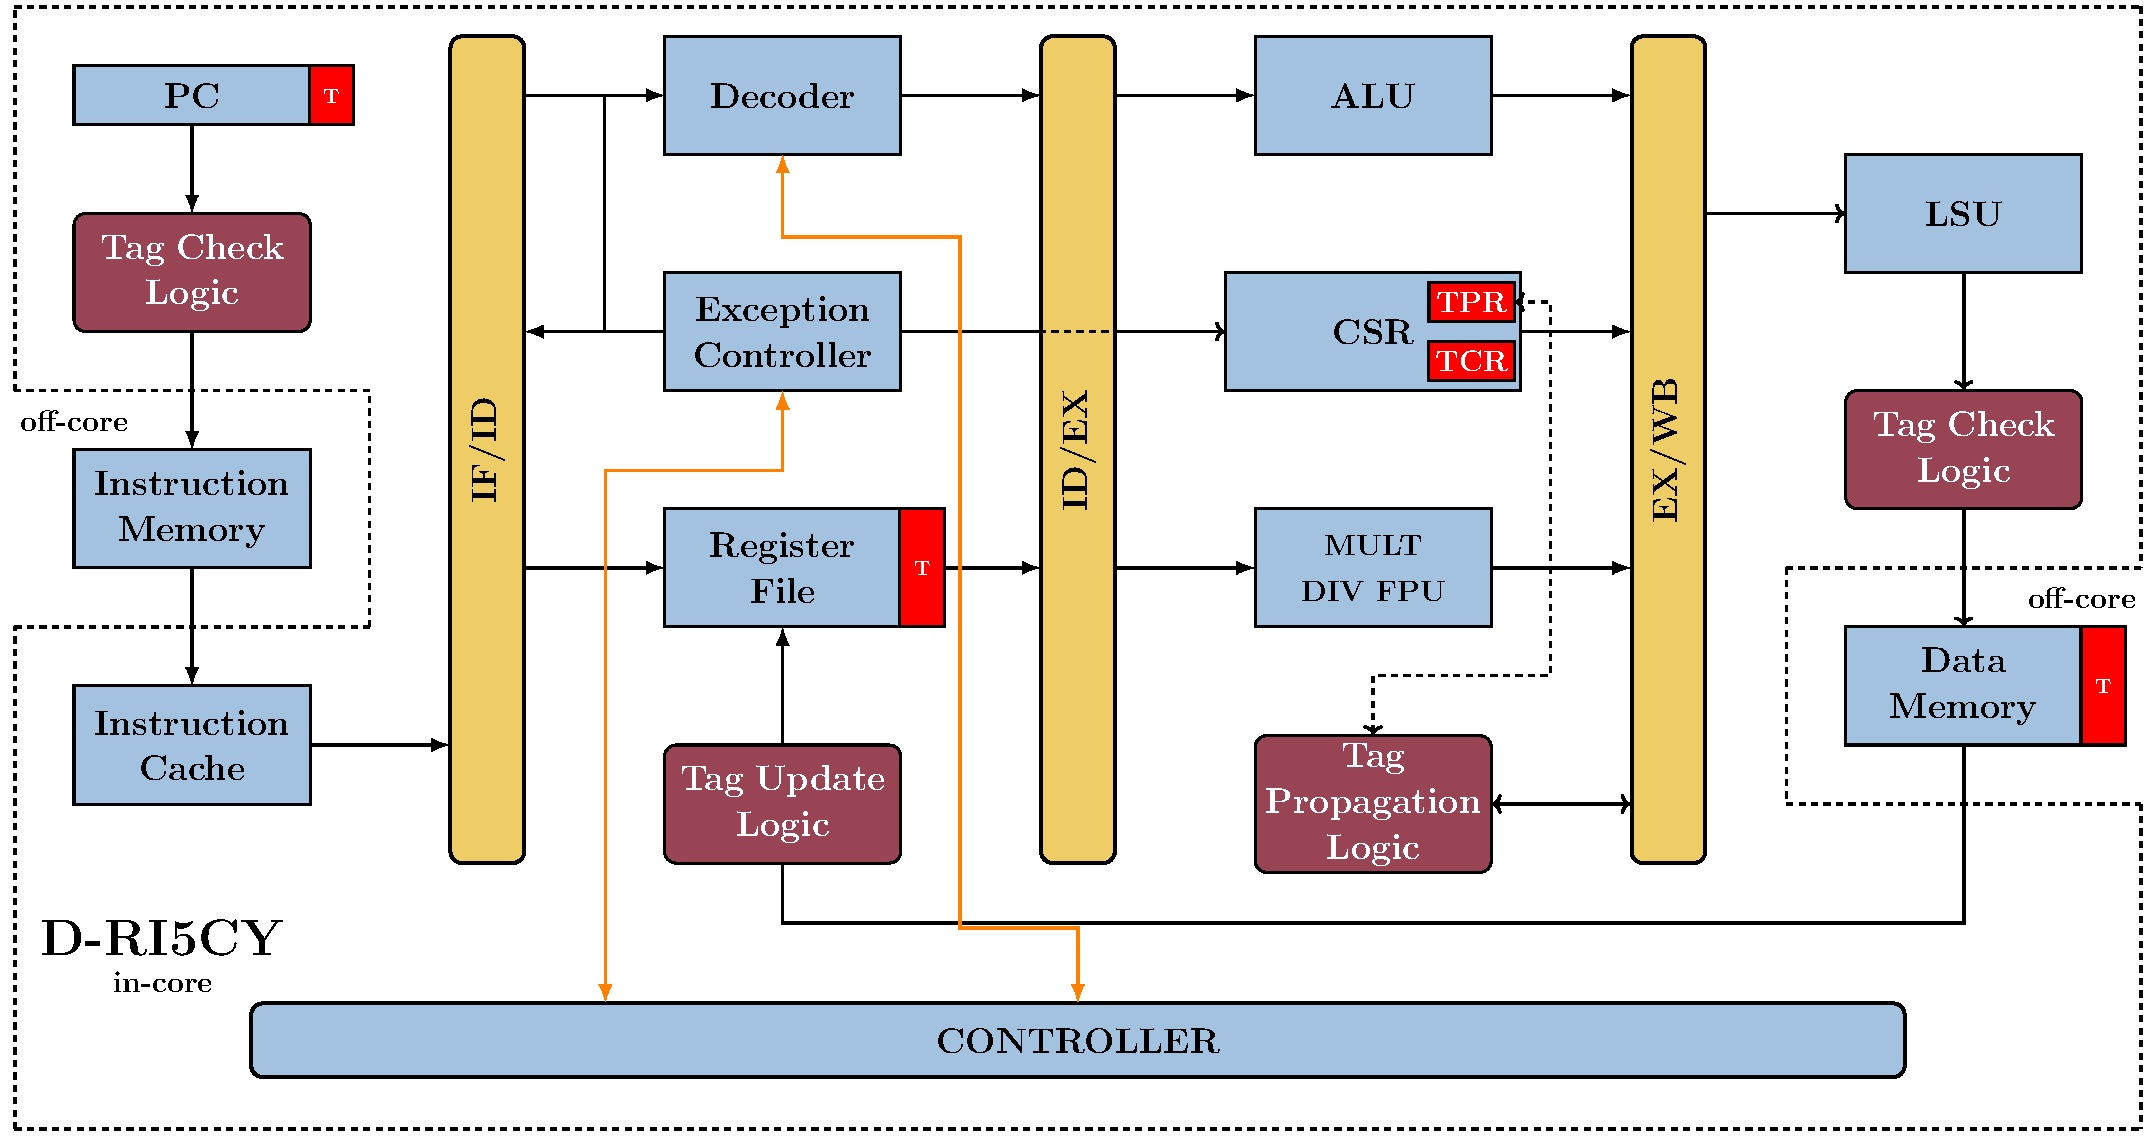
\includegraphics[width=.9\textwidth]{src/2_vuln_assessment/img/RI5CY.pdf}
        \caption{Architecture of the D-RI5CY.}
        \label{fig:riscy}
    \end{figure}
\end{frame}
%%%%%%%%%%%%%%%%%%%%%%%%%%%%%%%%%%%%%%%%%%%%%%%%%%%%%%%%%%%%%%%%%%%%%%%%%%%%
\subsection{Vulnerability assessment}
\begin{frame}{Vulnerability Assessment}
    \begin{block}{Threat model}
        We consider an attacker able to:
        \begin{itemize}
            \item perform a physical attack to defeat the DIFT mechanism and realise a software attack,
            \item inject faults in DIFT-related registers:
                  \begin{itemize}
                      \item bit set,
                      \item bit reset,
                      \item bit-flip.
                  \end{itemize}
        \end{itemize}
    \end{block}

    % \begin{block}{Methodology}
    %     \begin{itemize}
    %         \item Analysis of 2 attacks use cases: buffer overflow attack, format string attack
    %         \item Analysis of 1 use case to complete the DIFT surface: compare/compute
    %     \end{itemize}
    % \end{block}
\end{frame}
%%%%%%%%%%%%%%%%%%%%%%%%%%%%%%%%%%%%%%%%%%%%%%%%%%%%%%%%%%%%%%%%%%%%%%%%%%%%
\subsection{Use case : presentation}
\begin{frame}{Case 1: Buffer overflow}
    \begin{itemize}
        \item The attacker exploits a buffer overflow to access the return address register ($RA$).
    \end{itemize}

    \begin{figure}
        \centering
        \begin{subfigure}[l]{.45\textwidth}
            \centering
            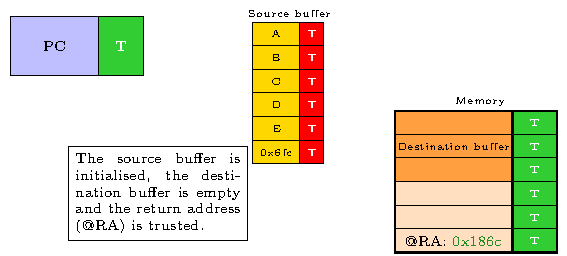
\includegraphics[width=.9\textwidth, page=1]{src/2_vuln_assessment/img/buffer_overflow/schemaPedagogique.pdf}
            \caption{Malicious buffer and $RA$ trusted}
            \label{fig:bo_1st_step}
        \end{subfigure}
        \begin{subfigure}[r]{.45\textwidth}
            \centering
            \includegraphics[width=.9\textwidth, page=5]{src/2_vuln_assessment/img/buffer_overflow/schemaPedagogique.pdf}
            \caption{Overflow and overwriting of $RA$ and its tag}
            \label{fig:bo_3rd_step}
        \end{subfigure}
    \end{figure}

    \begin{itemize}
        \item As the data in the source buffer is manipulated by the user, it is marked as \textcolor{red}{\textit{untrusted}}.
        \item Thanks to DIFT, the tags associated with the source buffer data overwrite the $RA$ register tag.
        \item When the function returns, the corrupted register $RA$ is loaded into $PC$ using a jalr instruction.
    \end{itemize}
\end{frame}

\begin{frame}
    \begin{figure}
        \centering
        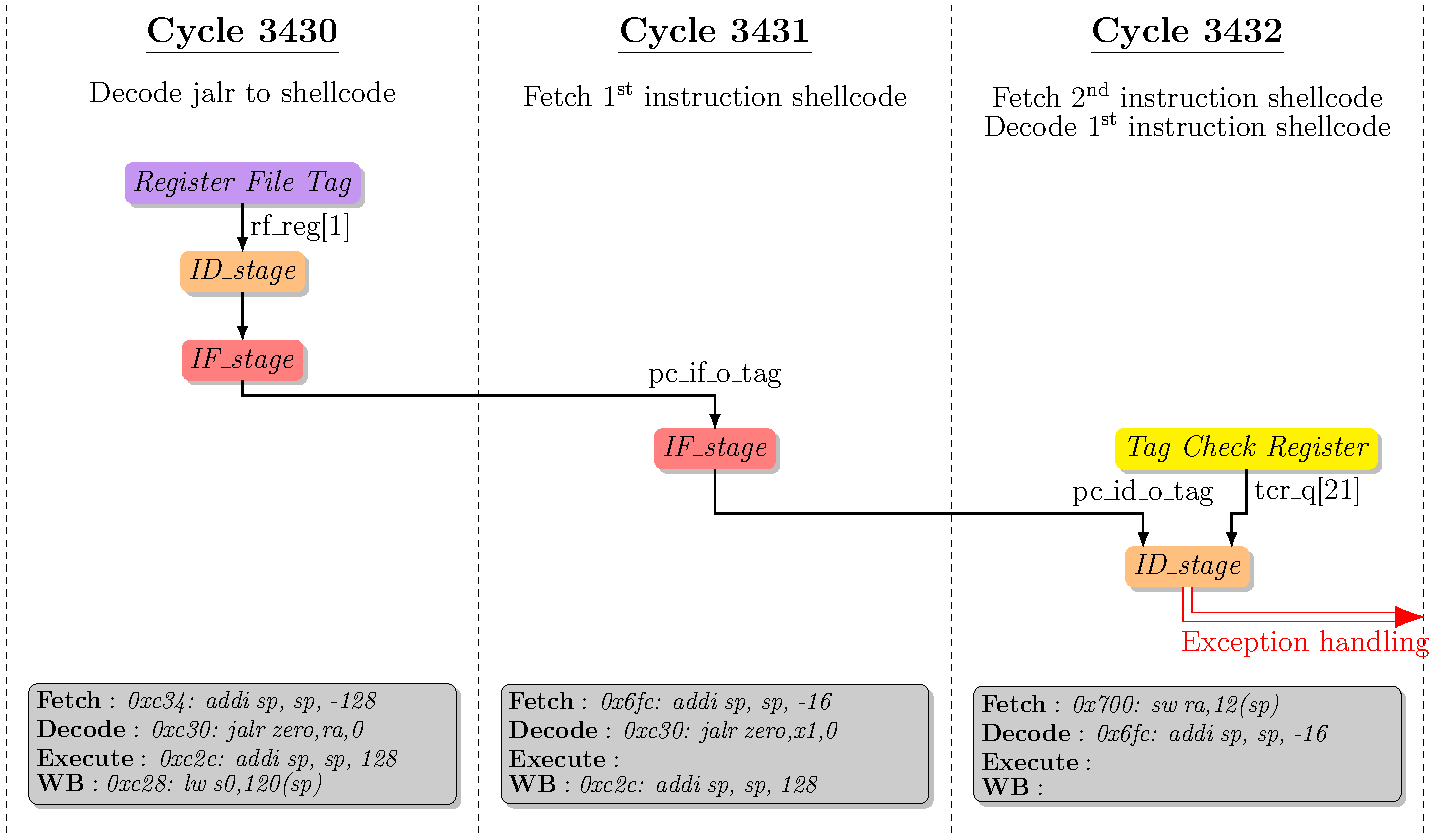
\includegraphics[width=.75\textwidth]{src/2_vuln_assessment/img/buffer_overflow/bufferOverflowAttack_short.pdf}
        \caption{Temporal analysis of the tags propagation in \textit{Buffer Overflow} attack}
        \label{fig:analyseTempoBufferOverflow}
    \end{figure}
\end{frame}

\begin{frame}
    \begin{figure}
        \centering
        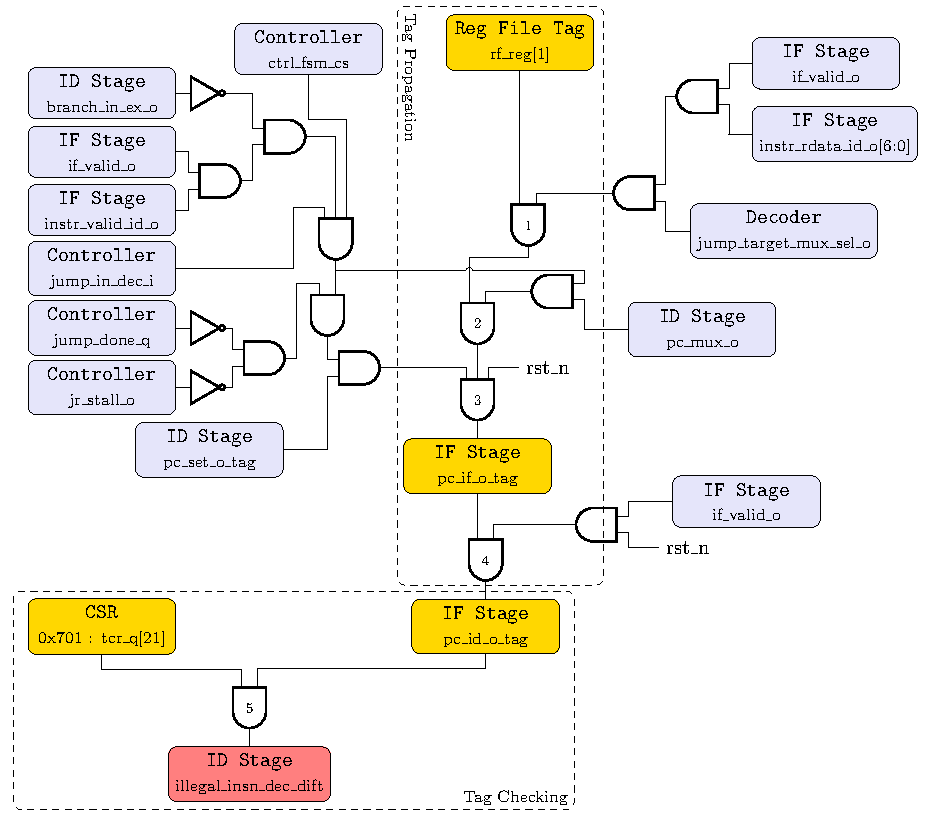
\includegraphics[height=.85\textheight]{src/2_vuln_assessment/img/buffer_overflow/arborescence_bufferOverflow.pdf}
        \caption{Logical analysis of the tags propagation in a \textit{Buffer Overflow} attack}
        \label{fig:analyseLogiqueBufferOverflow}
    \end{figure}
\end{frame}
%%%%%%%%%%%%%%%%%%%%%%%%%%%%%%%%%%%%%%%%%%%%%%%%%%%%%%%%%%%%%%%%%%%%%%%%%%%%%%%%%%%%%%%%%%%%%%%%%%%%%%%%%%%%
\begin{frame}[fragile]{Case 2: WU-FTPd}
    \begin{itemize}
        \justifying
        \item The vulnerability is the use of an unchecked user input as the format string parameter in functions that perform formatting, e.g. printf()
        \item An attacker can use the format tokens, to write into arbitrary locations of memory, e.g. the return address of the function.
    \end{itemize}

    % \vspace{1cm}
    % \hspace{2cm}
    \centering
    \begin{minipage}[c]{\textwidth}
        \begin{lstlisting}[language=C,label=code:printfNFormat]
void echo(){
    int a;
    register int i asm("x8");
    a = i;
    printf("%224u%n%35u%n%253u%n%n", 1, (int*) (a-4), 1, (int*) (a-3), 1, (int*) (a-2), (int*) (a-1));
}\end{lstlisting}
    \end{minipage}
\end{frame}

\begin{frame}
    \begin{figure}
        \centering
        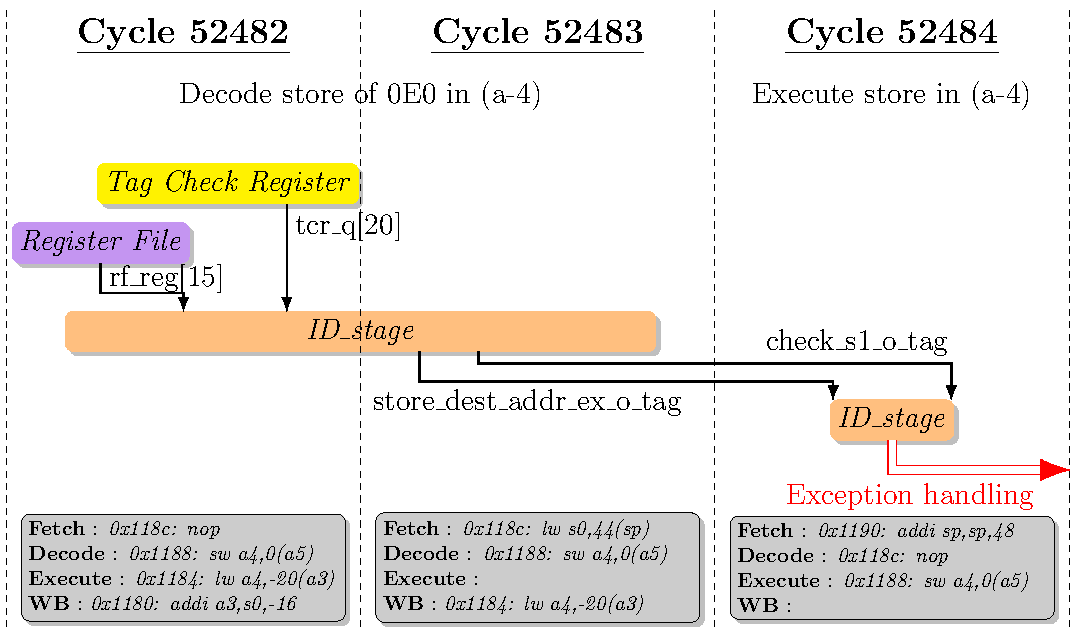
\includegraphics[height=.85\textheight]{src/2_vuln_assessment/img/wuftpd/ftpd_short.pdf}
        \caption{Temporal analysis of the tags propagation in a \textit{format string} attack}
        \label{fig:analyseTempoFormatString}
    \end{figure}
\end{frame}

\begin{frame}
    \begin{figure}
        \centering
        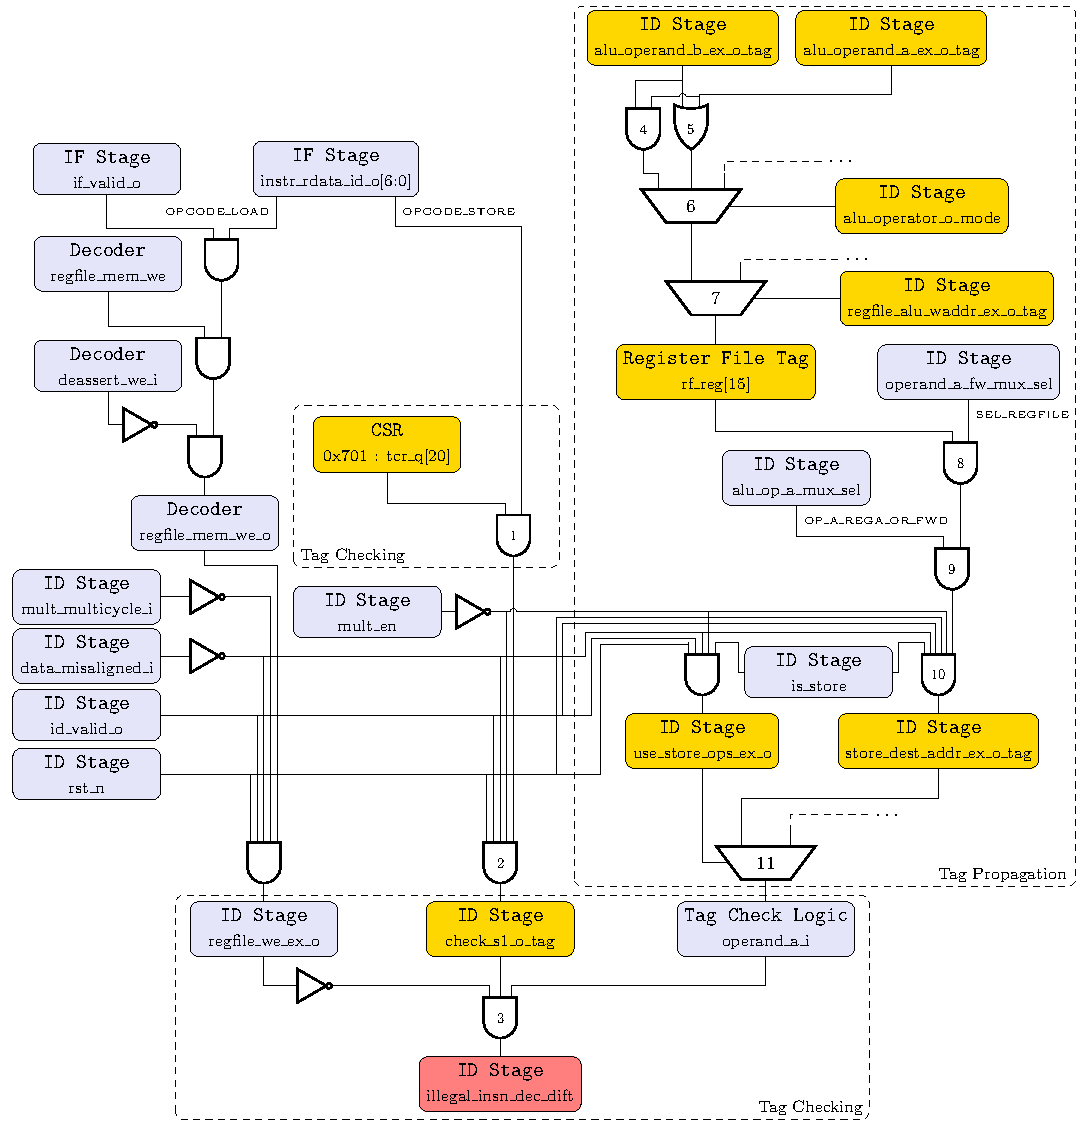
\includegraphics[height=.85\textheight]{src/2_vuln_assessment/img/wuftpd/arborescence_wuftpd.pdf}
        \caption{Logical analysis of the tags propagation in a \textit{format string} attack}
        \label{fig:analyseLogiqueFormatString}
    \end{figure}
\end{frame}
%%%%%%%%%%%%%%%%%%%%%%%%%%%%%%%%%%%%%%%%%%%%%%%%%%%%%%%%%%%%%%%%%%%%%%%%%%%%%%%%%%%%%%%%%%%%%%%%%%%%%%%%%%%%
\subsection{Experimental Setup}
%%%%%%%%%%%%%%%%%%%%%%%%%%%%%%%%%%%%%%%%%%%%%%%%%%%%%%%%%%%%%%%%%%%%%%%%%%%%%%%%%%%%%%%%%%%%%%%%%%%%%%%%%%%%
\begin{frame}{Experimental Setup - Simulation fault injections campaign}
    \begin{itemize}
        \justifying
        \item Logical fault injection simulation is used for preliminary evaluations
              \begin{itemize}
                  \justifying
                  \item faults are injected in the HDL code at cycle accurate and bit accurate level
                  \item a set of 55 DIFT-related registers are targeted
                  \item a reference simulation is done without fault
                  \item results are classed in four groups
                        \begin{itemize}
                            \justifying
                            \item crash: reference cycle count exceeded,
                            \item silent: current faulted simulation is the same as the reference simulation
                            \item delay: illegal instruction is delayed
                            \item success: DIFT has been bypassed
                        \end{itemize}
              \end{itemize}
        \item Simulations with QuestaSim 10.6e.
    \end{itemize}
\end{frame}
%%%%%%%%%%%%%%%%%%%%%%%%%%%%%%%%%%%%%%%%%%%%%%%%%%%%%%%%%%%%%%%%%%%%%%%%%%%%%%%%%%%%%%%%%%%%%%%%%%%%%%%%%%%%
\begin{frame}{Main results : 3 cases}
    \begin{table}[H]
        \centering
        \caption{End of simulation status}
        \label{table:end_sim_by_status}
        \begin{tabular}{lrrrlr}
            \toprule
                            & Crash & NSTR & Delay & Success     & Total \\
            \midrule
            Buffer overflow & 0     & 1380 & 20    & 22 (1.55\%) & 1422  \\
            WU-FTPd         & 0     & 1767 & 77    & 52 (2.74\%) & 1896  \\
            Compare/Compute & 0     & 917  & 12    & 19 (2.00\%) & 948   \\
            \bottomrule
        \end{tabular}
    \end{table}
\end{frame}

\begin{frame}{Buffer overflow}
    \begin{table}[]
        \centering
        \caption{Buffer overflow : Register sensitivity as determined by fault model and simulation time}
        \label{table:end_sim_from_time_fault_register_buffer_overflow}
        \resizebox{\textwidth}{!}{%
            \begin{tabular}{llllllllllllllll}
                \toprule
                                                & \multicolumn{3}{c}{Cycle 3428} & \multicolumn{3}{c}{Cycle 3429} & \multicolumn{3}{c}{Cycle 3430} & \multicolumn{3}{c}{Cycle 3431} & \multicolumn{3}{c}{Cycle 3432}                                                                                                                 \\\cmidrule(lr){2-4}\cmidrule(lr){5-7}\cmidrule(lr){8-10}\cmidrule(lr){11-13}\cmidrule(lr){14-16}
                                                & set0                           & set1                           & bitflip                        & set0                           & set1                           & bitflip    & set0       & set1 & bitflip    & set0       & set1 & bitflip    & set0       & set1 & bitflip    \\
                \midrule
                pc\_if\_o\_tag                  &                                &                                &                                &                                &                                &            &            &      &            & \checkmark &      & \checkmark &            &      &            \\
                rf\_reg[1]                      &                                &                                &                                &                                &                                &            & \checkmark &      & \checkmark &            &      &            &            &      &            \\
                tcr\_q                          & \checkmark                     &                                &                                & \checkmark                     &                                &            & \checkmark &      &            & \checkmark &      &            & \checkmark &      &            \\
                \rowcolor{LightGray} tcr\_q[21] &                                &                                & \checkmark                     &                                &                                & \checkmark &            &      & \checkmark &            &      & \checkmark &            &      & \checkmark \\
                tpr\_q                          & \checkmark                     & \checkmark                     &                                & \checkmark                     & \checkmark                     &            &            &      &            &            &      &            &            &      &            \\
                \rowcolor{LightGray} tpr\_q[12] &                                &                                & \checkmark                     &                                &                                & \checkmark &            &      &            &            &      &            &            &      &            \\
                \rowcolor{LightGray} tpr\_q[15] &                                &                                & \checkmark                     &                                &                                & \checkmark &            &      &            &            &      &            &            &      &            \\
                \bottomrule
            \end{tabular}
        }
    \end{table}
\end{frame}

\begin{frame}{Discussion}
    \begin{itemize}
        \setbeamertemplate{itemize items}[triangle]
        \item 4212 simulations have been performed,
        \item 93 successes (2.21\%),
        \item We have shown that the D-RI5CY DIFT is vulnerable to FIA
        \item Propagation of faults is facilitated by paths fully made of \textit{AND} gates
    \end{itemize}
\end{frame}
%%%%%%%%%%%%%%%%%%%%%%%%%%%%%%%%%%%%%%%%%%%%%%%%%%%%%%%%%%%%%%%%%%%%%%%%%%%%%%%%%%%%%%%%%%%%%%%%%%%%%%%%%%%%
	%
	% ---------------------------------------------------------------- %
	\section{Proposed protections against FIAs}


%%%%%%%%%%%%%%%%%%%%%%%%%%%%%%%%%%%%%%%%%%%%%%%%%%%%%%%%%%%%%%%%%%%%%%%%%%%%%%%%%%%%%%%%%%%%%%%%%%%%%%%%%%%%
\begin{frame}{Introduction}
    \begin{block}{Protections}
        \begin{itemize}
            \item We propose 3 lightweight countermeasures using parity codes
            \begin{itemize}
                \item Simple parity
                \item Hamming Code
                \item Hamming Code with an additional bit (SECDED)
            \end{itemize}
        \end{itemize}
    \end{block}
\end{frame}
%%%%%%%%%%%%%%%%%%%%%%%%%%%%%%%%%%%%%%%%%%%%%%%%%%%%%%%%%%%%%%%%%%%%%%%%%%%%%%%%%%%%%%%%%%%%%%%%%%%%%%%%%%%%
\subsection{Simple Parity}
    \begin{frame}{Detection of single-bit errors - Simple Parity}
        \begin{block}{}
            \begin{itemize}
                \justifying
                \item Focusing into lightweight protections for small systems
                \item Often used for error detection.
                \item Add an extra bit for parity computation.
                \item Can only detect one error without correction.
            \end{itemize}
        \end{block}

        \vfill
        
        \begin{figure}
            \centering
            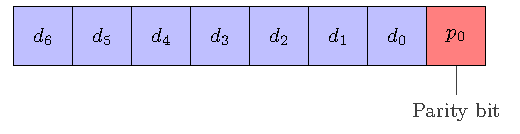
\includegraphics[width=.5\textwidth, page=1]{src/3_strategies/img/simple_parity.pdf}
            \caption{Simple parity codeword}
            \label{fig:simple_parity_codeword}
        \end{figure}
    \end{frame}

    \begin{frame}{Implementation - Simple Parity}
        \begin{figure}
            \centering
            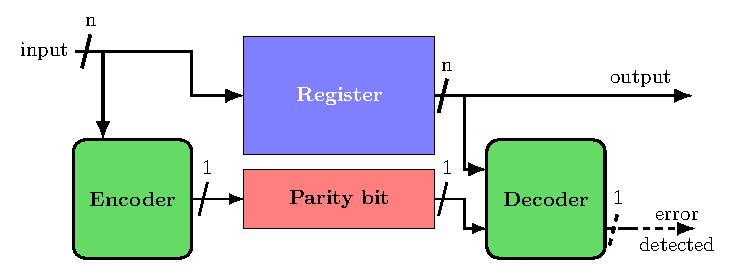
\includegraphics[width=\textwidth, page=1]{src/3_strategies/img/archi_contremesures.pdf}
            \caption{Simple Parity implementation}
            \label{fig:simple_parity_implem}
        \end{figure}
    \end{frame}
%%%%%%%%%%%%%%%%%%%%%%%%%%%%%%%%%%%%%%%%%%%%%%%%%%%%%%%%%%%%%%%%%%%%%%%%%%%%%%%%%%%%%%%%%%%%%%%%%%%%%%%%%%%%
\subsection{Hamming Code}
    \begin{frame}{Detection and correction of single-bit errors - Hamming Code}
        \begin{block}{}
            \begin{itemize}
                \justifying
                \item Linear error-correcting codes invented by Richard W. Hamming~\cite{H-50-bstj}.
                \item Mostly used in digital communication and data storage systems.
                \item Detect and correct single-bit error.
                \item Redundancy bits are placed in power of 2 positions.
                \item The number of redundancy bits depends on the number of bits to be protected {\scriptsize ($ 2^r \ge m + r + 1 $)}
            \end{itemize}
        \end{block}

        \begin{minipage}[c]{0.4\linewidth}
            \begin{equation} \label{equat:hamming_encoder}
                \begin{split}
                    r_{0} &= d_{0} \oplus d_{1} \oplus d_{3} \oplus d_{4} \oplus d_{6} \\
                    r_{1} &= d_{0} \oplus d_{2} \oplus d_{3} \oplus d_{5} \oplus d_{6} \\
                    r_{2} &= d_{1} \oplus d_{2} \oplus d_{3} \\
                    r_{3} &= d_{4} \oplus d_{5} \oplus d_{6}
                \end{split}
            \end{equation}
        \end{minipage}\hfill%
        \begin{minipage}[c]{0.55\linewidth}
            \begin{figure}
                \centering
                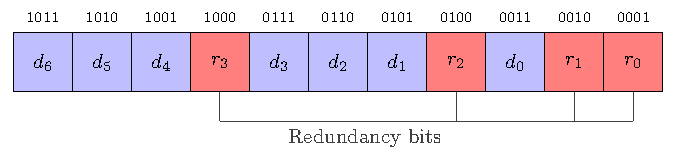
\includegraphics[width=\textwidth, page=1]{src/3_strategies/img/hamming_bit.pdf}
                \caption{Hamming codeword}
                \label{fig:hamming_codeword}
            \end{figure}
        \end{minipage}
    \end{frame}
    
    \begin{frame}{Implementation - Hamming Code}
        \begin{figure}
            \centering
            \includegraphics[width=.9\textwidth, page=2]{src/3_strategies/img/archi_contremesures.pdf}
            \caption{Hamming Code implementation for independant registers}
            \label{fig:hamming_code_implem_independant_register}
        \end{figure}
    \end{frame}
    
    \begin{frame}{Implementation - Hamming Code}
        \begin{figure}
            \centering
            \includegraphics[width=.9\textwidth, page=3]{src/3_strategies/img/archi_contremesures.pdf}
            \caption{Hamming Code implementation for Register File}
            \label{fig:hamming_code_implem_rf}
        \end{figure}
    \end{frame}
%%%%%%%%%%%%%%%%%%%%%%%%%%%%%%%%%%%%%%%%%%%%%%%%%%%%%%%%%%%%%%%%%%%%%%%%%%%%%%%%%%%%%%%%%%%%%%%%%%%%%%%%%%%%
\subsection{Hamming Code - SECDED}
\begin{frame}{Detection of two-bit errors and correction of single-bit errors - SECDED}
    \begin{block}{}
        \begin{itemize}
            \justifying
            \item Based on Hamming Code.
            \item Detect two-bit error and correct single-bit error.
            \item The number of redundancy bits depends on the number of bits to be protected {\scriptsize ($ 2^r \ge m + r + 1 $)}.
            \item An additional bit is placed at index 0, it is called: general parity bit
        \end{itemize}
    \end{block}

    \begin{minipage}[c]{0.4\linewidth}
        \begin{equation} \label{equat:secded_encoder}
            \begin{split}
                r_{0}  &= d_{0} \oplus d_{1} \oplus d_{3} \oplus d_{4} \oplus d_{6} \\
                r_{1}  &= d_{0} \oplus d_{2} \oplus d_{3} \oplus d_{5} \oplus d_{6} \\
                r_{2}  &= d_{1} \oplus d_{2} \oplus d_{3} \\
                r_{3}  &= d_{4} \oplus d_{5} \oplus d_{6} \\
                gp_{0} &= \bigoplus_{i=0}^{6} d_{i} \oplus \bigoplus_{j=0}^{3} r_{j}
            \end{split}
        \end{equation}
    \end{minipage}\hfill%
    \begin{minipage}[c]{0.6\linewidth}
        \begin{figure}
            \centering
            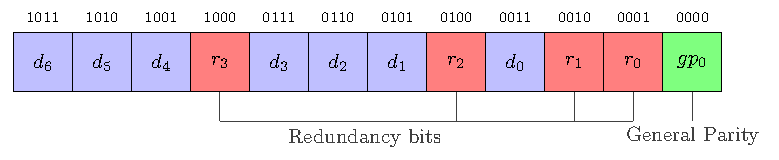
\includegraphics[width=\textwidth, page=1]{src/3_strategies/img/secded.pdf}
            \caption{SECDED codeword}
            \label{fig:secded_codeword}
        \end{figure}
    \end{minipage}
\end{frame}
    
\begin{frame}{Implementation - SECDED}
    \begin{figure}
        \centering
        \includegraphics[width=.8\textwidth, page=4]{src/3_strategies/img/archi_contremesures.pdf}
        \caption{SECDED implementation for independant registers}
        \label{fig:secded_implem_independant_register}
    \end{figure}
\end{frame}

\begin{frame}{Implementation - SECDED}
    \begin{figure}
        \centering
        \includegraphics[width=.9\textwidth, page=5]{src/3_strategies/img/archi_contremesures.pdf}
        \caption{SECDED implementation for Register File}
        \label{fig:secded_implem_rf}
    \end{figure}
\end{frame}
%%%%%%%%%%%%%%%%%%%%%%%%%%%%%%%%%%%%%%%%%%%%%%%%%%%%%%%%%%%%%%%%%%%%%%%%%%%%%%%%%%%%%%%%%%%%%%%%%%%%%%%%%%%%
\begin{frame}{Threat model}
    \begin{block}{Threat model}
        \begin{itemize}
            \item DIFT-related registers + protection-related registers
            \item Single bit-flip in one register
            \item Single bit-flip in two registers at two distinct clock cycles
            \item Single bit-flip in two registers at a given clock cycle
            \item Multi-bit faults in one register at a given clock cycle
            \item Multi-bit faults in two registers at a given clock cycle
        \end{itemize}
    \end{block}
\end{frame}
%%%%%%%%%%%%%%%%%%%%%%%%%%%%%%%%%%%%%%%%%%%%%%%%%%%%%%%%%%%%%%%%%%%%%%%%%%%%%%%%%%%%%%%%%%%%%%%%%%%%%%%%%%%%
\begin{frame}{Implemented strategies - Group composition}
    \begin{table}[t]
        \centering
        \caption{Grouping composition of implemented strategies}
        \label{tab:strategies_group}
        \begin{tabular}{@{}cccc@{}}
            \toprule
                       & Grouping composition                                 & Number of groups & Number of registers \\ \midrule
            Baseline   & --                                                   & --               & 55                  \\
            Strategy 1 & Minimisation of groups                               & 5                & 65                  \\
            Strategy 2 & Protection per pipeline stage                        & 7                & 69                  \\
            Strategy 3 & Protection per register                              & 24               & 103                 \\
            Strategy 4 & Protection per register with slicing of CSR & 38               & 131                 \\
            Strategy 5 & Coupling sliced registers                            & 39               & 133                 \\
            \bottomrule
        \end{tabular}
    \end{table}
\end{frame}
%%%%%%%%%%%%%%%%%%%%%%%%%%%%%%%%%%%%%%%%%%%%%%%%%%%%%%%%%%%%%%%%%%%%%%%%%%%%%%%%%%%%%%%%%%%%%%%%%%%%%%%%%%%%
\begin{frame}{Implemented strategies - details}
    \begin{table}[t]
        \centering
        \caption{Summary of DIFT-related protected registers -- taking SECDED}
        \label{tab:detail_strategies_group}
        \begin{tabular}{@{}cccccc@{}}
            \toprule
                       & \begin{tabular}[c]{@{}c@{}}Number of\\ protected bits\end{tabular} & \begin{tabular}[c]{@{}c@{}}Number of\\ redundancy bits\end{tabular} & \begin{tabular}[c]{@{}c@{}}Number of\\ parity bits\end{tabular} & \begin{tabular}[c]{@{}c@{}}Number of\\ bits\end{tabular} \\ \midrule
            Strategy 1 & 107                                                                & 25                                                                  & 5                                                               & 157                                                      \\
            Strategy 2 & 107                                                                & 30                                                                  & 7                                                               & 164                                                      \\
            Strategy 3 & 107                                                                & 64                                                                  & 24                                                              & 215                                                      \\
            Strategy 4 & 103                                                                & 101                                                                 & 38                                                              & 266                                                      \\
            Strategy 5 & 102                                                                & 114                                                                 & 39                                                              & 280                                                      \\
            \bottomrule
        \end{tabular}
    \end{table}
\end{frame}
%%%%%%%%%%%%%%%%%%%%%%%%%%%%%%%%%%%%%%%%%%%%%%%%%%%%%%%%%%%%%%%%%%%%%%%%%%%%%%%%%%%%%%%%%%%%%%%%%%%%%%%%%%%%
	%
	% ---------------------------------------------------------------- %
	\section{Experimental results}

%%%%%%%%%%%%%%%%%%%%%%%%%%%%%%%%%%%%%%%%%%%%%%%%%%%%%%%%%%%%%%%%%%%%%%%%%%%%
\begin{frame}{Experimental setup}
    
\end{frame}
%%%%%%%%%%%%%%%%%%%%%%%%%%%%%%%%%%%%%%%%%%%%%%%%%%%%%%%%%%%%%%%%%%%%%%%%%%%%
\begin{frame}{FPGA implementation results - Strategy 1}
    \begin{table}[t]
        \footnotesize
        \centering
        \caption{FPGA implementation results — Vivado 2023.2}
        \label{tab:chap5_implementation}
        \begin{tabular}{@{}c|ccc@{}}
            \toprule
            Protection    & Number of LUTs   & Number of FFs    & Maximum frequency                \\ \midrule
            Baseline      & 6,597 (-4.54\%) & 2,211 (-5.31\%) & \SI{49.1}{\mega\hertz} (3\%)     \\
            D-RI5CY       & 6,911 (0\%)     & 2,335 (0\%)     & \SI{47.6}{\mega\hertz} (0\%)     \\
            Simple parity & 7,011 (1.45\%)  & 2,337 (0.09\%)  & \SI{47.6}{\mega\hertz} (0\%)     \\
            Hamming Code  & 7,283 (5.38\%)  & 2,361 (1.11\%)  & \SI{47.4}{\mega\hertz} (-0.36\%) \\
            SECDED        & 7,428 (7.48\%)  & 2,366 (1.33\%)  & \SI{47.2}{\mega\hertz} (-0.95\%) \\
            \bottomrule
        \end{tabular}
    \end{table}
\end{frame}
%%%%%%%%%%%%%%%%%%%%%%%%%%%%%%%%%%%%%%%%%%%%%%%%%%%%%%%%%%%%%%%%%%%%%%%%%%%%%%%%%%%%%%%%%%%%%%%%%%%%%%%%%%%%
	%
	% ---------------------------------------------------------------- %
	\section{Conclusion and Perspectives}


%%%%%%%%%%%%%%%%%%%%%%%%%%%%%%%%%%%%%%%%%%%%%%%%%%%%%%%%%%%%%%%%%%%%%%%%%%%%
\subsection{Conclusion}

\begin{frame}{Conclusion}
    
\end{frame}

%%%%%%%%%%%%%%%%%%%%%%%%%%%%%%%%%%%%%%%%%%%%%%%%%%%%%%%%%%%%%%%%%%%%%%%%%%%%
\subsection{Perspectives}

\begin{frame}{Perspectives}
    
\end{frame}
%%%%%%%%%%%%%%%%%%%%%%%%%%%%%%%%%%%%%%%%%%%%%%%%%%%%%%%%%%%%%%%%%%%%%%%%%%%%
	%
	% ---------------------------------------------------------------- %
	\section*{Publications}

%%%%%%%%%%%%%%%%%%%%%%%%%%%%%%%%%%%%%%%%%%%%%%%%%%%%%%%%%%%%%%%%%%%%%%%%%%%%
\begin{frame}
    \vfill
    \centering
    \begin{beamercolorbox}[sep=8pt,center,shadow=true,rounded=true]{title}
        \usebeamerfont{section title} Publications
    \end{beamercolorbox}
    \vfill
\end{frame}

%%%%%%%%%%%%%%%%%%%%%%%%%%%%%%%%%%%%%%%%%%%%%%%%%%%%%%%%%%%%%%%%%%%%%%%%%%%%
\begin{frame}[noframenumbering]{Publications}

\end{frame}
%%%%%%%%%%%%%%%%%%%%%%%%%%%%%%%%%%%%%%%%%%%%%%%%%%%%%%%%%%%%%%%%%%%%%%%%%%%%
\begin{frame}
    \centering

    \vfill
    \begin{beamercolorbox}[sep=8pt,center,shadow=true,rounded=true]{title}
        \usebeamerfont{title}\NoHyper\large\inserttitle\par\endNoHyper
        \vspace{.5cm}
        \usebeamerfont{subtitle}\NoHyper\large\insertsubtitle\par\endNoHyper
    \end{beamercolorbox}
    \vfill

    \large \textbf{William PENSEC}

    \vfill

    \Large Thank you for your attention.

    \vfill
    
\includegraphics[height=1cm]{img/logo/ubs.png}
    \hspace{1cm}
    
\includegraphics[height=1cm]{img/logo/labsticc.pdf}
    \hspace{1cm}
    \includegraphics[height=1cm]{img/logo/cnrs.pdf}
\end{frame}
%%%%%%%%%%%%%%%%%%%%%%%%%%%%%%%%%%%%%%%%%%%%%%%%%%%%%%%%%%%%%%%%%%%%%%%%%%%%%%%%%%%%%%%%%%%%%%%%%%%%%%%%%%%%
	%
	% ---------------------------------------------------------------- %
	
\begin{frame}[noframenumbering]
    \vfill
    \centering
    \begin{beamercolorbox}[sep=8pt,center,shadow=true,rounded=true]{title}
        \usebeamerfont{section title} References
    \end{beamercolorbox}
    \vfill
\end{frame}

\begin{frame}[allowframebreaks, noframenumbering]{References}
    \printbibliography
\end{frame}
	%
	% ---------------------------------------------------------------- %
\end{document}
